

\chapter{Le compas éphémère}\label{c.collapse}



Un compas moderne est un compas fixe : la distance entre les deux branches peut être fixée de manière à pouvoir copier un segment  ou un cercle d'une position à une autre (fig.~\ref{fig.fixed-compass}). Euclide utilise un \og compas éphémère\fg{} qui ne permet pas de conserver  une distance fixe entre les branches  (fig.~\ref{fig.collapsing-compass}). Les enseignants utilisent souvent un compas éphémère constitué d'un marqueur attaché à une ficelle pour tracer un cercle sur un tableau blanc. Il est impossible de maintenir une longueur fixe lorsque le compas est retiré du tableau blanc. 

Ce chapitre commence par une discussion sur la pertinence de l'étude de la construction avec une règle et un compas (sect.~\ref{s.relevance}).
Dans la section~\ref{s.collapse}, on  compare les deux types de compas dans la construction la plus élémentaire, celle d'une médiatrice. La section~\ref{s.collapse-copy} présente la méthode d'Euclide pour copier un segment  à l'aide d'un compas éphémère. Cela montre que toute construction qui peut être réalisée à l'aide d'un compas fixe peut l'être à l'aide d'un compas éphémère. La section~\ref{s.collapse-copy-incorrect} présente  une démonstration de ce théorème qui semble correcte, mais qui ne fonctionne pas pour toutes les configurations de droites et de points. Pour souligner qu'il ne faut pas se fier aux figures, la section~\ref{s.collapse-isoceles} présente une célèbre fausse démonstration  que tous les triangles sont isocèles; la démonstration  semble correcte mais ne l'est pas car elle est basée sur une figure qui n'est pas correcte.

%\vspace{0.4cm}

\begin{minipage}{0.4\textwidth}
\centering
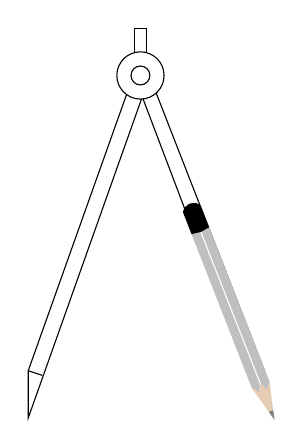
\begin{tikzpicture}
\begin{scope}[rotate=0,transform shape,scale=3]
\draw (2.95,3.7) rectangle (3,3.95);
\draw (2.92,3.68) -- (2.5,2.5) -- (2.5,2.3) -- (2.99,3.68);
\draw (3.5,2.5) -- (3.43,2.48) -- (2.975,3.68);
\draw (3.04,3.68) -- (3.5,2.5);
\draw (2.5,2.5) -- (2.56,2.48);
\draw[fill=white] (2.975,3.75) circle (0.1cm);
\draw (2.975,3.75) circle (0.04cm);
\end{scope}
\begin{scope}[xshift=10.34cm,yshift=7.28cm,rotate=21.4,scale=.6]          
\fill[gray!50] (0,4) -- (0.4,4) -- (0.4,0) --
               (0.3,-0.15) -- (0.2,0) -- (0.1,-0.14) --
               (0,0) -- cycle;
\draw[color=white] (0.2,4) -- (0.2,0);
\fill[black] (0,3.5) -- (0.2,3.47) -- (0.4,3.5) --
             (0.4,4) arc(30:150:0.23cm);
\fill[brown!40] (0,0) -- (0.2,-0.8)
    node[coordinate,pos=0.75](a){} -- 
    (0.4,0)node[coordinate,pos=0.25](b){} -- 
    (0.3,-0.15) -- (0.2,0) -- (0.1,-0.14) -- cycle;
\fill[gray] (a) -- (0.2,-0.8) -- (b) -- cycle;
\end{scope}
\end{tikzpicture}
%\includegraphics[width=0.8\textwidth]{Fig1_1a}
         \captionof{figure}{Un compas fixe. Une branche est munie d'une pointe que l'on place au centre du cercle. Un crayon fixé à l'autre branche est utilisé pour tracer le cercle. Les branches sont reliées par une articulation  serrée de sorte que la distance entre les branches (le rayon du cercle) est maintenue même lorsqu'on soulève le compas  du papier.}
         \label{fig.fixed-compass}
     \end{minipage}\hspace{3em}
     \begin{minipage}{0.4\textwidth}
         \centering
         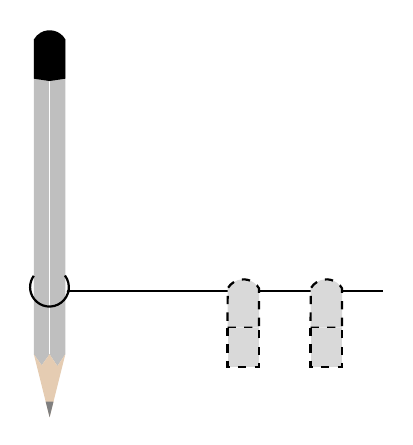
\begin{tikzpicture}[rotate=0,scale=1]          
\fill[gray!50] (0,4) -- (0.4,4) -- (0.4,0) --
               (0.3,-0.15) -- (0.2,0) -- (0.1,-0.14) --
               (0,0) -- cycle;
\draw[color=white] (0.2,4) -- (0.2,0);
\fill[black] (0,3.5) -- (0.2,3.47) -- (0.4,3.5) --
             (0.4,4) arc(30:150:0.23cm);
\fill[brown!40] (0,0) -- (0.2,-0.8)
    node[coordinate,pos=0.75](a){} -- 
    (0.4,0) node[coordinate,pos=0.25](b){} -- 
    (0.3,-0.15) -- (0.2,0) -- (0.1,-0.14) -- cycle;
\fill[gray] (a) -- (0.2,-0.8) -- (b) -- cycle;

\draw[thick] (0.395,1) arc (37:-216:7pt);
\coordinate (knot) at (0.44,.8);
\draw[thick] (knot) -- +(4,0);
\fill (knot) circle (.7pt);

\begin{scope}[xshift=100pt,yshift=-90pt]
\draw[dashed,thick,fill=white!70!gray] (0,3.5) -- (0.4,3.5) -- 
      (0.4,4) arc(30:150:0.23cm) -- cycle;
\draw[dashed,thick,fill=white!70!gray] (0,3.5) -- ++(0,-.5) -- ++(.4,0) -- ++(0,.5);
\end{scope}

\begin{scope}[xshift=70pt,yshift=-90pt]
\draw[dashed,thick,fill=white!70!gray] (0,3.5) -- (0.4,3.5) -- 
      (0.4,4) arc(30:150:0.23cm) -- cycle;
\draw[dashed,thick,fill=white!70!gray] (0,3.5) -- ++(0,-.5) -- ++(.4,0) -- ++(0,.5);
\end{scope}
\end{tikzpicture}
%\includegraphics[width=0.8\textwidth]{Fig1_1b}
         \captionof{figure}{Un compas éphémère. L'utilisateur tient un morceau de ficelle au centre du cercle. L'autre extrémité de la ficelle est attachée à un crayon et est utilisée pour tracer le cercle. Lorsqu'on soulève le compas  du papier, les doigts (en pointillés) peuvent facilement glisser vers une nouvelle position.}      \label{fig.collapsing-compass}
     \end{minipage}

%\vspace{0.4cm}




\section{Construction à la règle et au  compas}\label{s.relevance}

La construction à la règle et au compas était autrefois le concept fondamental enseigné en géométrie euclidienne. Récemment, elle est tombée en désuétude dans les programmes scolaires. Il est vrai que ce sujet n'a que peu, voire pas, d'utilité pratique. Comme nous le montrons dans les sections~\ref{s.neusis}, \ref{s.neusis-doubling}, \ref{s.q} et  \ref{s.square-quad}, les Grecs savaient réaliser des constructions impossibles avec la règle et le compas en utilisant des outils à peine plus sophistiqués. Aujourd'hui, grâce à des méthodes numériques, les ordinateurs peuvent réaliser ces constructions avec toute la précision souhaitée.

Néanmoins, je pense qu'il y a des avantages à étudier ces constructions :
\begin{itemize}
\item Il est plus amusant et plus stimulant d'apprendre la géométrie par des constructions que par la simple lecture de théorèmes et de démonstrations.
\item D'importantes percées en mathématiques ont été réalisées en tentant de trouver de telles constructions. Le chapitre~\ref{c.heptadecagon} présente une construction de Gauss qui a conduit à l'algèbre abstraite moderne, en particulier à la théorie développée par \'Evariste Galois.
\item Il est quelque peu contre-intuitif et donc très intéressant de pouvoir démontrer qu'il est impossible de construire certains objets géométriques.
\item Malheureusement, de nombreuses personnes perdent des années de leur vie à essayer de réaliser des constructions impossibles. Les étudiants devraient certainement être conscients de la futilité de pareils efforts.
\end{itemize}

\section{Les compas fixes et les compas éphémères}\label{s.collapse}

Certains manuels de géométrie présentent la construction de la médiatrice  d'un segment  en construisant deux cercles de même rayon centrés aux extrémités du segment de sorte que le rayon soit supérieur ou égal   à la moitié de la longueur du segment (fig.~\ref{f.collapse-perp-bisector-fixed}). Cette opération ne peut être réalisée qu'avec un compas fixe, car après avoir tracé le cercle de centre  $A$, la distance entre les branches du compas doit rester fixe pour tracer le cercle de centre $B$.


\vspace{0.4cm}

\begin{minipage}{0.4\textwidth}
\centering   
\begin{tikzpicture}[scale=0.5]
\coordinate (A) at (0,0);
\coordinate (B) at (4,0);
\vertex{A};
\vertex{B};
\draw (A) node[below left] {$A$} -- (B) node[below right] {$B$};
\draw[name path=larc] (A) ++(-60:3cm) arc (-60:60:3cm);
\draw[name path=rarc] (B) ++(-120:3cm) arc (-120:-240:3cm);
\path [name intersections={of=larc and rarc,by={b,t}}];
\node[above right,xshift=-2pt,yshift=5pt] at (t) {$C$};
\node[below left,xshift=2pt,yshift=-5pt] at (b) {$D$};
\draw ($ (b) ! 1.2 ! (t)$) -- ($ (t) ! 1.2 ! (b)$);
\end{tikzpicture}
%\includegraphics[width=0.8\textwidth]{Fig1_2a}
         \captionof{figure}{Construction d'une médiatrice avec un compas fixe.}
         \label{f.collapse-perp-bisector-fixed}
     \end{minipage}
     \hspace{3em}
     \begin{minipage}{0.4\textwidth}
\centering   
\begin{tikzpicture}[scale=0.4]
\coordinate (A) at (0,0);
\coordinate (B) at (4,0);
\vertex{A};
\vertex{B};
\draw (A) node[below left] {$A$} -- (B) node[below right] {$B$};
\draw[name path=larc] (A) ++(-80:4cm) arc (-80:80:4cm);
\draw[name path=rarc] (B) ++(-100:4cm) arc (-100:-260:4cm);
\path [name intersections={of=larc and rarc,by={b,t}}];
\node[above right,xshift=-2pt,yshift=3pt] at (t) {$C$};
\node[below left,xshift=2pt,yshift=-3pt] at (b) {$D$};
\draw ($ (b) ! 1.2 ! (t)$) -- ($ (t) ! 1.2 ! (b)$);
\end{tikzpicture}
%\includegraphics[width=0.6\textwidth]{Fig1_2b}
         \captionof{figure}{Construction d'une médiatrice  à l'aide d'un compas fixe ou d'un compas éphémère.}
         \label{f.collapse-perp-bisector-collapse}
     \end{minipage}

\vspace{0.4cm}


La figure~\ref{f.collapse-perp-bisector-collapse} montre la construction d'une médiatrice  avec un compas fixe ou avec un compas éphémère. On construit deux cercles : un cercle de centre $A$ avec un rayon  $\overline{AB}$ et un cercle de centre $B$ avec un rayon  $\overline{BA}$. Ceci peut être fait avec un compas éphémère car  évidemment  $\overline{AB}=\overline{BA}$, donc le compas n'a pas besoin de \og se souvenir\fg{} de la longueur de $\overline{AB}$ pour construire un cercle de centre $B$ avec le même rayon.
La démonstration que la droite construite  dans la figure~\ref{f.collapse-perp-bisector-fixed} est la médiatrice  n'est pas du tout élémentaire car des concepts relativement avancés comme les triangles isométriques doivent être utilisés. Cependant, la démonstration  que la construction d'une médiatrice  illustrée dans la figure~\ref{f.collapse-perp-bisector-collapse} est correcte est simple et repose sur le fait que $\triangle ABC$  est un triangle équilatéral. C'est d'ailleurs la première proposition des \emph{Éléments} d'Euclide. 
$\overline{AC}=\overline{AB}$ puisque ce sont des rayons d'un même cercle et, de même, $\overline{BC}=\overline{BA}$. On a donc : $
\overline{AC}=\overline{AB}=\overline{BA}=\overline{BC}$.

La figure~\ref{f.collapse-equilateral-fixed} montre que pour la construction avec un compas fixe, le triangle sera un triangle isocèle et pas nécessairement un triangle équilatéral (fig.~\ref{f.collapse-equilateral-collapse}).



\begin{minipage}{0.4\textwidth}
\centering  
\begin{tikzpicture}[scale=0.5]
\coordinate (A) at (0,0);
\coordinate (B) at (4,0);
\vertex{A};
\vertex{B};
\draw (A) node[below left] {$A$} -- (B) node[below right] {$B$};
\draw[name path=larc] (A) ++(-60:3cm) arc (-60:60:3cm);
\draw[name path=rarc] (B) ++(-120:3cm) arc (-120:-240:3cm);
\path [name intersections={of=larc and rarc,by={b,t}}];
\vertex{t};
\vertex{b};
\node[above right,xshift=-2pt,yshift=5pt] at (t) {$C$};
\node[below left,xshift=2pt,yshift=-5pt] at (b) {$D$};
\draw (A) -- (t);
\draw (B) -- (t);
\end{tikzpicture}
%\includegraphics[width=0.8\textwidth]{Fig1_3a}
         \captionof{figure}{Construction d'un triangle isocèle avec un compas fixe.}
         \label{f.collapse-equilateral-fixed}
         
     \end{minipage}
     \hspace{3em}
     \begin{minipage}{0.4\textwidth}
\centering      
\begin{tikzpicture}[scale=0.5]
\coordinate (A) at (0,0);
\coordinate (B) at (4,0);
\draw (A) node[below left] {$A$} -- (B) node[below right] {$B$};
\vertex{A};
\vertex{B};
\draw[name path=larc] (A) ++(-80:4cm) arc (-80:80:4cm);
\draw[name path=rarc] (B) ++(-100:4cm) arc (-100:-260:4cm);
\path [name intersections={of=larc and rarc,by={b,t}}];
\vertex{t};
\vertex{b};
\node[above right,xshift=-2pt,yshift=3pt] at (t) {$C$};
\node[below left,xshift=2pt,yshift=-3pt] at (b) {$D$};
\draw (A) -- (t);
\draw (B) -- (t);
\end{tikzpicture}
%\includegraphics[width=0.7\textwidth]{Fig1_3b}
         \captionof{figure}{Construction d'un triangle équilatéral avec un compas  éphémère.}
         \label{f.collapse-equilateral-collapse}
     \end{minipage}



\section{Construction d'Euclide pour copier un segment}\label{s.collapse-copy}

La deuxième proposition des \emph{Éléments} d'Euclide décrit comment copier un segment  donné $\overline{AB}$ en un segment de même longueur, dont l'une des  extrémités  est un point donné $C$. Par conséquent, un compas fixe n'ajoute aucune capacité supplémentaire. Un compas éphémère est suffisant, bien que les constructions soient plus faciles avec un compas fixe.

\begin{theorem}
Étant donné un segment $\overline{AB}$ et un point $C$, on peut construire un segment $\overline{CC'}$  à l'aide d'un compas éphémère de sorte que $\overline{AB}=\overline{CC'}$ (fig.~\ref{f.collapse-copying-1}).
\end{theorem}

\vspace{0.4cm}

\begin{minipage}{0.42\textwidth}
\centering     
\begin{tikzpicture}[scale=0.5]
\coordinate (C) at (0,0);
\coordinate (A) at (3,0);
\draw (A) node[below,xshift=-2pt,yshift=-2pt] {$A$} -- +(40:4) coordinate (B) node[right] {$B$};
\vertex{A};
\vertex{B};
\vertex{C};
\node[below,xshift=2pt,yshift=-2pt] at (C) {$C$};
\draw[thick,dashed] (C) -- +(160:4) coordinate (D) node[below] {$C'$};
\vertex{D};
\end{tikzpicture}
%\includegraphics[width=\textwidth]{Fig1_4a}
         \captionof{figure}{Copie du segment  $\overline{AB}$. L'orientation de $\overline{CC'}$ n'est pas importante.}
         \label{f.collapse-copying-1}
     \end{minipage}
     \hspace{3em}
     \begin{minipage}{0.42\textwidth}
\centering    
\begin{tikzpicture}[scale=0.5]
\coordinate (C) at (0,0);
\coordinate (A) at (3,0);
\draw (A) node[below,xshift=-2pt,yshift=-2pt] {$A$} -- +(40:4) coordinate (B) node[right] {$B$};
\vertex{B};
\node[below,xshift=2pt,yshift=-2pt] at (C) {$C$};
\draw (A) -- (C);
\path[name path=larc] (C) ++(-70:2.5cm) arc (-70:70:2.5cm);
\path[name path=rarc] (A) ++(-110:2.5cm) arc (-110:-250:2.5cm);
\path [name intersections={of=larc and rarc,by={d,D}}];
\node[above] at (D) {$D$};
\draw (A) -- (D);
\draw (C) -- (D);
\end{tikzpicture}
%\includegraphics[width=0.8\textwidth]{Fig1_4b}
         \captionof{figure}{Copie d'un segment  avec un compas éphémère.}
         \label{f.collapse-copying-2}
     \end{minipage}


\vspace{0.4cm}


\begin{proof}
Traçons le segment  $\overline{AC}$. Construisons le triangle équilatéral $\triangle ACD$ dont la base est $\overline{AC}$ (fig.~\ref{f.collapse-copying-2}). D'après la première proposition d'Euclide, le triangle peut être construit à l'aide d'un compas éphémère. Construisons la demi-droite  qui prolonge le segment  de $D$ à $A$, et construisons la demi-droite qui  prolonge le segment  de $D$ à $C$  (fig.~\ref{f.collapse-copying-3}). Construisons le cercle de centre $A$ et de  rayon $\overline{AB}$. Soit $E$  l'intersection du cercle et de la demi-droite qui prolonge $\overline{DA}$ 
 (fig.~\ref{f.collapse-copying-4}). Construisons le cercle de centre  $D$ et de  rayon  $\overline{DE}$. Soit $F$  l'intersection de ce cercle et de la demi-droite qui prolonge $\overline{DC}$  (fig.~\ref{f.collapse-copying-5}).

\vspace{0.4cm}

\begin{minipage}{0.4\textwidth}
\centering    
\begin{tikzpicture}[scale=0.4]
\coordinate (C) at (0,0);
\coordinate (A) at (3,0);
\draw (A) node[below,xshift=-2pt,yshift=-2pt] {$A$} -- +(40:4) coordinate (B) node[right] {$B$};
\node[below,xshift=2pt,yshift=-2pt] at (C) {$C$};
\draw (A) -- (C);
\path[name path=larc] (C) ++(-70:2.5cm) arc (-70:70:2.5cm);
\path[name path=rarc] (A) ++(-110:2.5cm) arc (-110:-250:2.5cm);
\path [name intersections={of=larc and rarc,by={d,D}}];
\node[above] at (D) {$D$};
\draw (A) -- (D);
\draw (C) -- (D);
\draw[name path=ray2] (D) -- ($ (D) ! 3 ! (C) $);
\draw[name path=ray1] (D) -- ($ (D) ! 3 ! (A) $);
\end{tikzpicture}
%\includegraphics[width=\textwidth]{Fig1_5a}
         \captionof{figure}{Construction de demi-droites à partir de~$D$.}
   \label{f.collapse-copying-3}
     \end{minipage}
     \hspace{3em}
     \begin{minipage}{0.4\textwidth}
\centering   
\begin{tikzpicture}[scale=0.4]
\coordinate (C) at (0,0);
\coordinate (A) at (3,0);
\draw (A) node[below,xshift=-2pt,yshift=-2pt] {$A$} -- +(40:4) coordinate (B) node[right] {$B$};
\node[below,xshift=2pt,yshift=-2pt] at (C) {$C$};
\draw (A) -- (C);
\path[name path=larc] (C) ++(-70:2.5cm) arc (-70:70:2.5cm);
\path[name path=rarc] (A) ++(-110:2.5cm) arc (-110:-250:2.5cm);
\path [name intersections={of=larc and rarc,by={d,D}}];
\node[above] at (D) {$D$};
\draw (A) -- (D);
\draw (C) -- (D);
\draw[name path=ray2] (D) -- ($ (D) ! 3 ! (C) $);
\draw[name path=ray1] (D) -- ($ (D) ! 3 ! (A) $);
\node[draw,circle through=(B),name path=c1] at (A) {};
\path [name intersections={of=c1 and ray1,by={E,e}}];
\node[right,xshift=2pt,yshift=-2pt] at (E) {$E$};
\end{tikzpicture}
%\includegraphics[width=\textwidth]{Fig1_5b}
         \captionof{figure}{Construction d'un cercle de rayon~$\overline{AB}$.}
         \label{f.collapse-copying-4}
     \end{minipage}

\vspace{0.4cm}



$\overline{DC}=\overline{DA}$ car $\triangle ACD$ est équilatéral. $\overline{AE}=\overline{AB}$ sont des rayons du même cercle, tout comme $\overline{DF}=\overline{DE}$. Par conséquent :
\[
\overline{CF}=\overline{DF}-\overline{DC}=\overline{DE}-\overline{DC}=\overline{DE}-\overline{DA}=\overline{AE}=\overline{AB}\,.\qedhere
\]
\end{proof}

\begin{figure}[htbp]
\centering
\begin{tikzpicture}[scale=0.4]
\clip (-5,-4.5) rectangle (8,6);
\coordinate (C) at (0,0);
\coordinate (A) at (3,0);
\draw (A) node[below,xshift=-2pt,yshift=-2pt] {$A$} -- +(40:4) coordinate (B) node[right] {$B$};
\node[below,xshift=2pt,yshift=-2pt] at (C) {$C$};
\draw (A) -- (C);
\path[name path=larc] (C) ++(-70:2.5cm) arc (-70:70:2.5cm);
\path[name path=rarc] (A) ++(-110:2.5cm) arc (-110:-250:2.5cm);
\path [name intersections={of=larc and rarc,by={d,D}}];
\node[above] at (D) {$D$};
\draw (A) -- (D);
\draw (C) -- (D);
\draw[name path=ray2] (D) -- ($ (D) ! 3 ! (C) $);
\draw[name path=ray1] (D) -- ($ (D) ! 3 ! (A) $);
\node[draw,circle through=(B),name path=c1] at (A) {};
\path [name intersections={of=c1 and ray1,by={E,e}}];
\node[right,xshift=2pt,yshift=-2pt] at (E) {$E$};
\node[draw,circle through=(E),name path=c2] at (D) {};
\path [name intersections={of=c2 and ray2,by={F,f}}];
\node[left,xshift=-2pt,yshift=-2pt] at (F) {$F$};
\path (A) -- node[right] {$a$} (E);
\path (C) -- node[left] {$a$} (F);
\draw[white,fill=white] (-5,4.5) rectangle +(13,1.5);
\end{tikzpicture}
%         \includegraphics[height=4cm]{Fig1_6.jpg}
     \caption{Construction de $\overline{CF}=\overline{AB}$.}
     \label{f.collapse-copying-5}
\end{figure}


La spécification des directions des demi-droites est essentielle. La démonstration fonctionne ici pour tout segment  $\overline{AB}$ et tout point $C$, quelle que soit sa position par rapport à $\overline{AB}$.  En spécifiant les directions, le \og cône\fg{} délimité par les deux demi-droites intersectera les cercles même si $\overline{AC}>\overline{AB}$ (fig.~\ref{f.collapse-copying-6}).

\begin{figure}[htbp]
\centering
\begin{tikzpicture}[scale=0.4]
\clip (-12,-6) rectangle (11,10);
\coordinate (C) at (-4,0);
\coordinate (A) at (3,0);
\draw (A) node[below,xshift=-2pt,yshift=-2pt] {$A$} -- +(40:4) coordinate (B) node[right] {$B$};
\node[below,xshift=2pt,yshift=-2pt] at (C) {$C$};
\draw (A) -- (C);
\path[name path=larc] (C) ++(-70:7cm) arc (-70:70:7cm);
\path[name path=rarc] (A) ++(-110:7cm) arc (-110:-250:7cm);
\path [name intersections={of=larc and rarc,by={d,D}}];
\node[above] at (D) {$D$};
\draw (A) -- (D);
\draw (C) -- (D);
\draw[name path=ray2] (D) -- ($ (D) ! 2 ! (C) $);
\draw[name path=ray1] (D) -- ($ (D) ! 2 ! (A) $);
\node[draw,circle through=(B),name path=c1] at (A) {};
\path [name intersections={of=c1 and ray1,by={e,E}}];
\node[right,xshift=2pt,yshift=-2pt] at (E) {$E$};
\node[draw,circle through=(E),name path=c2] at (D) {};
\path [name intersections={of=c2 and ray2,by={F,f}}];
\node[left,xshift=-2pt,yshift=-2pt] at (F) {$F$};
\path (A) -- node[right] {$a$} (E);
\path (C) -- node[left] {$a$} (F);
\draw[white,fill=white] (-12,8) rectangle +(23,2);
\end{tikzpicture}
%        \includegraphics[height=4cm]{Fig1_7.jpg}
        \caption{Construction si  $\overline{AC}>\overline{AB}$.}
        \label{f.collapse-copying-6}	
\end{figure}



\section[Une construction erronée pour copier un segment]{Une construction erronée pour copier un segment}\label{s.collapse-copy-incorrect}

\begin{proof}
Construisons trois cercles : un 
 cercle de centre  $A$ et de rayon $\overline{AB}$, un cercle de centre   $A$ et de rayon $\overline{AC}$ et un cercle de centre $C$ et de rayon $\overline{AC}=\overline{CA}$. Soient  $E$ et $F$ les intersections des cercles  de centres  $A$ et $C$ et de même rayon.  Soit $D$  une intersection du cercle de centre $C$ et du cercle de centre $A$ et de rayon $\overline{AB}$. Si $\overline{AC}>\overline{AB}$, la construction est celle de la figure~\ref{f.collapse-incorrect-1}.

\begin{figure}[htbp]
\centering
\begin{tikzpicture}[scale=0.5]
\coordinate (C) at (-2,0);
\coordinate (A) at (2.5,0);
\coordinate (B) at (4.5,1.5);
\draw (A) node[below right] {$A$} -- (B) node[right] {$B$};
\node[left,xshift=-2pt] at (C) {$C$};
\node[draw,circle through=(B),name path=c1] at (A) {};
\node[draw,circle through=(C),name path=c2] at (A) {};
\node[draw,circle through=(A),name path=c3] at (C) {};
\path [name intersections={of=c1 and c3,by={D,f}}];
\path [name intersections={of=c2 and c3,by={E,F}}];
\node[below right,xshift=4pt] at (D) {$D$};
\node[above,yshift=2pt] at (E) {$E$};
\node[below,yshift=-2pt] at (F) {$F$};
\vertex{C};
\end{tikzpicture}
%    \includegraphics[height=4.5cm]{Fig1_8.jpg}
     \caption{Construction pour la copie d'un segment  (1).}
    \label{f.collapse-incorrect-1}
\end{figure}

\begin{figure}[htbp]
\centering
\begin{tikzpicture}[scale=0.5]
\clip (-8,-1) rectangle (9,5);
\coordinate (C) at (-2,0);
\coordinate (A) at (2.5,0);
\coordinate (B) at (4.5,1.5);
\draw[thick] (A) node[below right] {$A$} -- (B) node[right] {$B$};
\vertex{A};
\vertex{C};
\node[below left] at (C) {$C$};
\node[draw,circle through=(B),name path=c1] at (A) {};
\node[draw,circle through=(C),name path=c2] at (A) {};
\node[draw,circle through=(A),name path=c3] at (C) {};
\path [name intersections={of=c1 and c3,by={D,f}}];
\path [name intersections={of=c2 and c3,by={E,F}}];
\node[draw,circle through=(D),name path=c4] at (E) {};
\path [name intersections={of=c2 and c4,by={g,G}}];
\node[left] at (G) {$G$};
\node[below right,yshift=2pt,xshift=2pt] at (D) {$D$};
\node[above] at (E) {$E$};
\vertex{E};
\vertex{F};
\draw (C) -- (G);
\draw (A) -- (G) -- (E) -- (C) -- (D);
\draw (A) -- (D) -- (E) -- cycle;
\end{tikzpicture}
%    \includegraphics[height=4.5cm]{Fig1_9.jpg}
     \caption{Construction pour la copie d'un segment  (2).}
    \label{f.collapse-incorrect-2}
\end{figure}



Construisons un cercle de centre $E$ et de rayon $\overline{ED}$. Soit $G$ l'intersection de ce cercle avec le cercle de centre $A$ et de rayon $\overline{AC}$. Il existe deux intersections, on choisit donc celle qui est la plus proche de $C$ (fig.~\ref{f.collapse-incorrect-2}).
$\overline{CD}=\overline{CE}$ sont des rayons du même cercle. De même,  $\overline{AE}=\overline{AG}$. Par construction, les rayons $\overline{CE}$ et $\overline{AE}$ sont égaux. Par conséquent,
\[
\overline{CD} = \overline{CE} = \overline{AE} = \overline{AG}\,.
\]
$\overline{EG} = \overline{ED}$ sont des rayons du même cercle, donc $\triangle EAG\cong \triangle DCE$ car les trois côtés sont les mêmes et $\angle GEA = \angle DEC$.



Puisque
\[
\angle GEC = \angle GEA \!-\!\angle CEA = \angle DEC\!-\!\angle CEA = \angle DEA\,,
\] 
il s'ensuit que $\triangle ADE\cong\triangle CGE$ d'après l'un des cas d'égalité des triangles (deux côtés et un angle égaux). $\overline{AB}=\overline{AD}$ sont des rayons du petit cercle de  centre  $A$, donc $\overline{GC}=\overline{AD}=\overline{AB}$.
\end{proof}

La démonstration n'est correcte que si $\overline{AC}>\overline{AB}$.  La figure~\ref{f.collapse-incorrect-4} montre un cas où $\overline{AC}<\overline{A}B$. On peut voir que $\overline{AB}\neq\overline{GC}$.

\begin{figure}[htbp]
\centering
\begin{tikzpicture}[scale=0.5]
\coordinate (C) at (-1,0);
\coordinate (A) at (2,0);
\coordinate (B) at (6,1.5);
\draw[thick] (A) node[below right] {$A$} -- (B) node[right] {$B$};
\node[left,xshift=-2pt] at (C) {$C$};
\node[draw,circle through=(B),name path=c1] at (A) {};
\node[draw,circle through=(C),name path=c2] at (A) {};
\node[draw,circle through=(A),name path=c3] at (C) {};
\path [name intersections={of=c1 and c3,by={D,f}}];
\path [name intersections={of=c2 and c3,by={E,F}}];
\node[above left,xshift=4pt] at (D) {$D$};
\node[above,yshift=2pt] at (E) {$E$};
\node[below,yshift=-2pt] at (F) {$F$};
\vertex{A};
\vertex{C};
\node[draw,circle through=(D),name path=c4] at (E) {};
\path [name intersections={of=c2 and c4,by={g,G}}];
\node[right,xshift=2pt,yshift=2pt] at (G) {$G$};
\draw[thick] (G) -- (C);
\end{tikzpicture}
%        \includegraphics[height=4.5cm]{Fig1_10.jpg}
     \caption{Un cas où la démonstration ne fonctionne pas.}
     \label{f.collapse-incorrect-4}
\end{figure}



\section{Ne vous fiez pas à une figure}\label{s.collapse-isoceles}

\begin{theorem} [faux bien sûr]
Tous les triangles sont isocèles.
\end{theorem}

\vspace{-2ex}

\begin{proof}[Démonstration fausse]
Pour un triangle arbitraire $\triangle ABC$, soit $P$ l'intersection de la bissectrice de l'angle $\angle BAC$ et de la médiatrice de $\overline{BC}$. Les intersections des hauteurs issues de $P$ avec les côtés $\overline{AB}$ et  $\overline{AC}$ sont désignées respectivement par $E$ et $F$ (fig.~\ref{f.collapse-isoceles-1}). 

\begin{figure}[htbp]
\centering
\begin{tikzpicture}[scale=1]
\coordinate (P) at (0,0);
\node[xshift=4mm,yshift=1mm] at (P) {$P$};
\coordinate [label=left:$B$] (B)  at (-2,-2);
\coordinate [label=right:$C$] (C)  at (4,-2);
\coordinate [label=above:$A$] (A)  at (-1,2);
\node[below,yshift=-12pt,xshift=1pt] at (A) {$\alpha$};
\node[below,yshift=-12pt,xshift=13pt] at (A) {$\alpha$};
\draw (A) -- (B);
\draw (A) -- (C);
\draw (B) -- (C);
\draw (A) -- (P);
\draw (B) -- (P);
\draw (C) -- (P);
\coordinate[label=left:$E$] (E) at ($ (A) ! .44 ! (B) $);
\draw[rotate=-100] (E) rectangle +(6pt,6pt);
\draw (P) -- (E);
\coordinate (F) at ($ (A) ! .33 ! (C) $);
\node[right,xshift=2pt,yshift=2pt] at (F) {$F$};
\draw[rotate=-132] (F) rectangle +(6pt,6pt);
\draw (P) -- (F);
\coordinate[label=below:$D$] (D) at ($ (B) ! .33 ! (C) $);
\draw (D) rectangle +(6pt,6pt);
\draw (P) -- (D);
\node[left] at ($ (A) ! .5 ! (E) $) {};
\node[left] at ($ (B) ! .5 ! (E) $) {};
\node[below] at ($ (B) ! .5 ! (D) $) {$a$};
\node[below] at ($ (C) ! .5 ! (D) $) {$a$};
\node[right,xshift=2pt] at ($ (A) ! .5 ! (F) $) {};
\node[right,xshift=2pt] at ($ (C) ! .5 ! (F) $) {};
\vertex{P};
\end{tikzpicture}
%        \includegraphics[height=4.5cm]{Fig1_11.jpg}
     \caption{Une démonstration  fausse que tous les triangles sont isocèles.}
     \label{f.collapse-isoceles-1}
\end{figure}





$\triangle APE\cong \triangle APF$ car ce sont des triangles rectangles avec des angles égaux $\alpha$ et un côté commun $\overline{AP}$. $\triangle DPB\cong \triangle DPC$ car ce sont des triangles rectangles, $\overline{PD}$ est un côté commun et $\overline{BD}=\overline{CD}=a$. $\triangle EPB\cong \triangle FPC$ car ce sont des triangles rectangles, $\overline{EP}=\overline{PF}$ d'après le premier couple de triangles  isométriques et $\overline{PB}=\overline{PC}$ d'après le second couple. En combinant les équations, on obtient que $\triangle ABC$ est isocèle :
\[
\overline{AB}= \overline{AE}+\overline{EB}=\overline{AF}+\overline{FC} =\overline{AC}\,.
\qedhere\]
\end{proof}

La logique de la démonstration est correcte, mais la figure sur laquelle  se base la démonstration n'est pas correcte car le point $P$ est à l'extérieur du triangle (fig.~\ref{f.collapse-isoceles-2}).

\begin{figure}[htbp]
\centering
\begin{tikzpicture}[scale=.5]
\coordinate (B) at (0,0);
\coordinate (C) at (8,0);
\path[name path=ba] (B) -- +(70:6);
\path[name path=ca] (C) -- +(140:8.5);
\path [name intersections={of=ba and ca,by={A}}];
\draw (B) -- (C) -- (A) -- cycle;
\node[above] at (A) {$A$};
\node[below,yshift=-12pt,xshift=-1pt] at (A) {$\alpha$};
\node[below right,xshift=5pt,yshift=-12pt] at (A) {$\alpha$};
\node[left] at (B) {$B$};
\node[right] at (C) {$C$};
\draw[name path=angle] (A) -- +(-75:9);
\draw ($(B)!.5!(C)$) -- +(0,3);
\draw[name path=perp] ($(B)!.5!(C)$) -- +(0,-3.5);
\path [name intersections={of=angle and perp,by={X}}];
\vertex{X};
\draw (4,0) rectangle +(10pt,10pt);
\node[right] at (X) {$P$};
\end{tikzpicture}
%        \includegraphics[height=4.5cm]{Fig1_12.jpg}
     \caption{Pourquoi la construction ne fonctionne pas.}
      \label{f.collapse-isoceles-2}
\end{figure}




\subsection*{Quelle est la surprise?}

En tant qu'élève, je considérais comme acquis qu'un compas possède une articulation qui maintient la distance entre la pointe et le crayon lorsqu'on le soulève du papier. Lorsque le professeur utilisait un compas fabriqué à partir d'une ficelle et d'un morceau de craie, je n'imaginais pas qu'il était différent de mon compas. L'article de Gotfried Toussaint a été une vraie surprise, tout comme son explication que les démonstrations post-euclidiennes n'étaient pas  correctes parce qu'elles dépendaient de figures qui faisaient des suppositions injustifiées. Je recommande cet article aux lecteurs qui souhaitent approfondir leur compréhension des démonstrations en mathématiques.

\subsection*{Sources}

Ce chapitre se base sur \cite{toussaint}. La construction inexacte de l'équivalence des deux compas dans la section~\ref{s.collapse-copy-incorrect} provient de \cite{rusty}. Bernard Vitrac a fait paraître une nouvelle  traduction française  des \emph{Éléments} d'Euclide, accompagnée d'un commentaire détaillé \cite{euclid}.

